%%%%%%%%%%%%%%%%%%%%%%%%%%%%%%%%%%%%%%%%%%%%%%%%%%%%%%%%%%%%%%%%%%%%%%%%%%%%%%%%
%2345678901234567890123456789012345678901234567890123456789012345678901234567890
%        1         2         3         4         5         6         7         8

\documentclass[letterpaper, 10 pt, conference]{ieeeconf}  % Comment this line out
                                                          % if you need a4paper
%\documentclass[a4paper, 10pt, conference]{ieeeconf}      % Use this line for a4
                                                          % paper

\IEEEoverridecommandlockouts                              % This command is only
                                                          % needed if you want to
                                                          % use the \thanks command
\overrideIEEEmargins
% See the \addtolength command later in the file to balance the column lengths
% on the last page of the document



% The following packages can be found on http:\\www.ctan.org
\usepackage{graphicx} % for pdf, bitmapped graphics files
\usepackage[hidelinks]{hyperref}
\usepackage{float}
\usepackage[section]{placeins}
%\usepackage{epsfig} % for postscript graphics files
%\usepackage{mathptmx} % assumes new font selection scheme installed
%\usepackage{times} % assumes new font selection scheme installed
%\usepackage{amsmath} % assumes amsmath package installed
%\usepackage{amssymb}  % assumes amsmath package installed

\title{\LARGE \bf
BIF 701 LAB 10: Using \href{https://www.omicsnet.ca/}{OmicsNet} to Explore Biological Networks
}

%\author{ \parbox{3 in}{\centering Huibert Kwakernaak*
%         \thanks{*Use the $\backslash$thanks command to put information here}\\
%         Faculty of Electrical Engineering, Mathematics and Computer Science\\
%         University of Twente\\
%         7500 AE Enschede, The Netherlands\\
%         {\tt\small h.kwakernaak@autsubmit.com}}
%         \hspace*{ 0.5 in}
%         \parbox{3 in}{ \centering Pradeep Misra**
%         \thanks{**The footnote marks may be inserted manually}\\
%        Department of Electrical Engineering \\
%         Wright State University\\
%         Dayton, OH 45435, USA\\
%         {\tt\small pmisra@cs.wright.edu}}
%}

\author {\href{https://www.linkedin.com/in/christopher-eeles-430b8a168/}{Christopher Eeles}}

\begin{document}

\maketitle
\thispagestyle{empty}
\pagestyle{empty}

%%%%%%%%%%%%%%%%%%%%%%%%%%%%%%%%%%%%%%%%%%%%%%%%%%%%%%%%%%%%%%%%%%%%%%%%%%%%%%%%
\begin{abstract}

In this laboratory we will explore the recently published web-tool from McGill researchers Zhou, G. and Xia, J. (2018), aptly named OmicsNet. Our survey of this tool and its functionalities will provide insight into the cutting edge of biological network creation, analysis and visualization software. In doing so we will outline the types of analyses possible using OmicsNet and conduct a thorough investigation of one such metholodology.

\end{abstract}

%%%%%%%%%%%%%%%%%%%%%%%%%%%%%%%%%%%%%%%%%%%%%%%%%%%%%%%%%%%%%%%%%%%%%%%%%%%%%%%%
\section{INTRODUCTION}

Previously developed biological network tools mainly focused on protein-pretion interaction (PPI) or metabolic networks and were often unable to handle high node volume without visualization becoming crowded and unreadable.$^3$ In response to these limitations OmicsNet was developed to allow simple biological network creation from a diverse set of molecular interactions for analysis and visualization in 3D space.$^3$ The tool is able to handle data sets from genes, proteins, microRNA, transcription factors and metabolites which can be combined and merged in a variety of ways.$^3$ 

Given the increasing importance of systems biology in understanding how complex interteractions create and affect the biology of cells, tissues, organisms and ecosystems, utilizing available network analysis tools and developing new ones is a necessity for bioinformaticians.$^2$ The possibilities in this field are vast, encompassing fields as diverse as biophysics and molecular physiology to epidemiology and ecology. Applications include development of prescision medicines, mapping complex webs of drug-drug interactions, interpreting correlations between genetic variants and disease, and myriad other endeavors in basic as well as applied biological and medical sciences.$^4$

\section{METHODS$^5$}

\subsection{\href{https://www.omicsnet.ca/}{OmicsNet}}

OmicsNet enables researchers to create networks to visualize relationships between genes, proteins, transcription factors and metabolites in 3D space. The web-tool contains a comprehensive, built-in knowledgebase allowing selection of multiple lists of molecules pertinent to a researcher's interets. Other data formats accepted include molecular lists--- wherein the first column is read as the input type and the second column is read as the expression or quantitative measurement---and network files with .sif, .txt and .graphml extensions. The web-app is supported accross multiple browswer including Chrome, Firefox and Safari with graphics generated using the WebGL Javascript API. Network generation starts from inputted molecular lists, which are then compared to the selected external interaction database to build the interaction network. The results are displayed in a highly customizable Javascript application which enables exploration using different network models, annotated and colourized by the user.

\subsection{Input Types}

We began by selecting each of the gene/proteins, transcription factors (TF), miRNAs, and graph file options on the OmicsNet main page. Firstly, the gene/proteins option allowed selection of organism species as well as an extensive list of available database ID formats for upload to the server; in this exploration we will simply use the example set provided by OmicsNet. Secondly the transcription factors option displayed a similar input window species and database ID options specific to that tool. This pattern continued for the remaining options, allowing us to conclude that input types vary only in species for anlaysis and databases available. The exception was the graph file option, which instead prompted us for a file to upload or example files for small (.txt) and large (.graphml) networks. 

\subsection{Network Building}

Examining the network building page we observed that concurrent input of gene, TF, miRNA and metabolite data was possible, but only three interactions could be selected at one time. Available interaction options inculde PPI, miRNA-gene interactions (MGI), metabolite-protein interactiong (MPI) and TF-gene interactions (TGI) each of which had interaction database options. Netwrok tools were also available to filter the input data to control network size. On submit, the network results summarize generated subnetworks, lising the number of nodes, edges and seeds for each.

\subsection{Network Viewer}

Proceeding to the network viewer, a Javascript interface displayed a visualization of our selected inputs and interactions. Input types were colourized with a legend available underneath which a node explorer, to select a subset of molecules of interest, allowed searching and deleting nodes based on the direction of your analysis. Edges appear to represent the relationships between nodes and can be customized for opacity to focus on each aspect respectively. Three layouts---spherical, force-directed and layered---allow different geometries to explore the networks relationships. To the right a number of explorer windows appear to allow more specific network analysis.

\subsection{Detailed Analysis}

For this lab we have select example data from Uniprot for protein and Kegg ID for metabolites, both for \emph{H. sapiens}. Two comparisons were selected, PPI and MPI respectively, using the default interaction databases. On submission we were prompted to select an approach to expand the primary PPI network, from which 'target primary seed nodes' was chosen. No network tools were used to modify network size. Exploration of the network viewer will be recorded in the results section for subsequent analysis and discussion.

\section{RESULTS$^5$}

The output labelled our proteins as genes, assumingly because our selected proteins are a result of expression these genes. Metabolites were highlighted in yellow. Edges were displayed in red and were bundled under the 'Edge' drop-down menu. Seed highlighting was also enabled to focus on the subset which was used to generate the network. Node labels were set to green for more easy visualization. Visualizations of the spherical, layered, and force-direction geometries are displayed in Fig. 1, Fig. 2 and Fig. 3, respectively.

\begin{figure}[h!]
    \centering

    \fbox{
        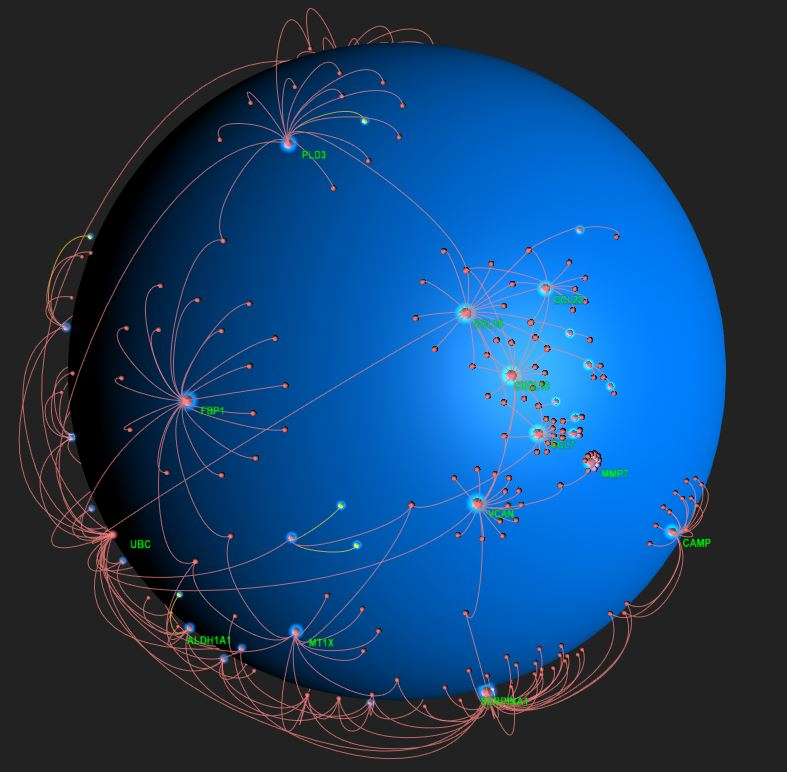
\includegraphics[width=3in]{Sphere.JPG}
    }
    \caption{Spherical Geometry}

\end{figure}


\begin{figure}[h!]
    \centering

    \fbox{
        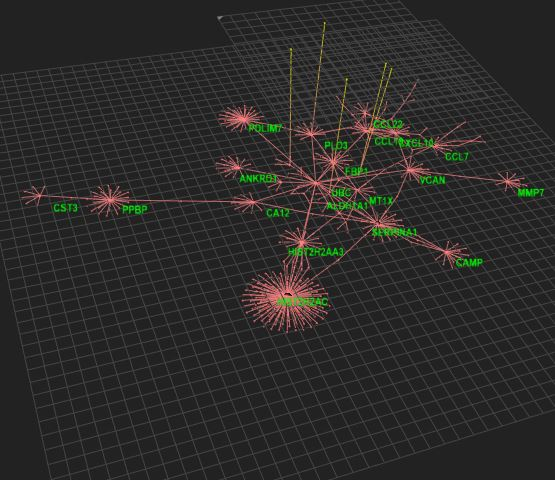
\includegraphics[width=3in]{Lay.JPG}
    }
    \caption{Layered Geometry}
\end{figure}



\begin{figure}[h!]
    \centering

    \fbox{
        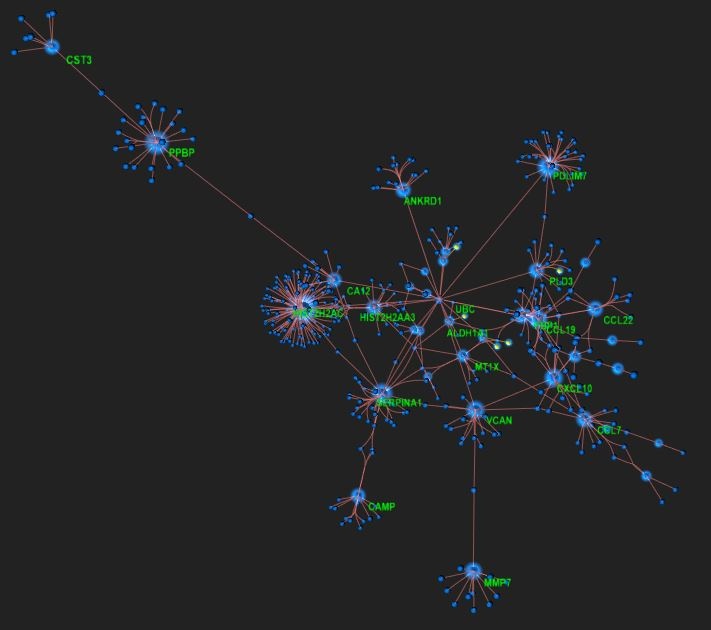
\includegraphics[width=3in]{FD.JPG}
    }
    \caption{Force-Direction Geometry}
\end{figure}


To explore the biological interpretation of these visualizations the HIST2HAC protein was selected due to its voluminous cluser of interactions. The HIST2H2AC protein and a subset of nodes---SMN1, TCF20 and ATXN7---were selected for indentification via the Uniprot database. The Fig. 4 displays the cluster selected, with the nodes of interest labelled and highlighted in blue. The batch selection function was used for this purpose.

\begin{figure}[h!]
    \centering

    \fbox{
        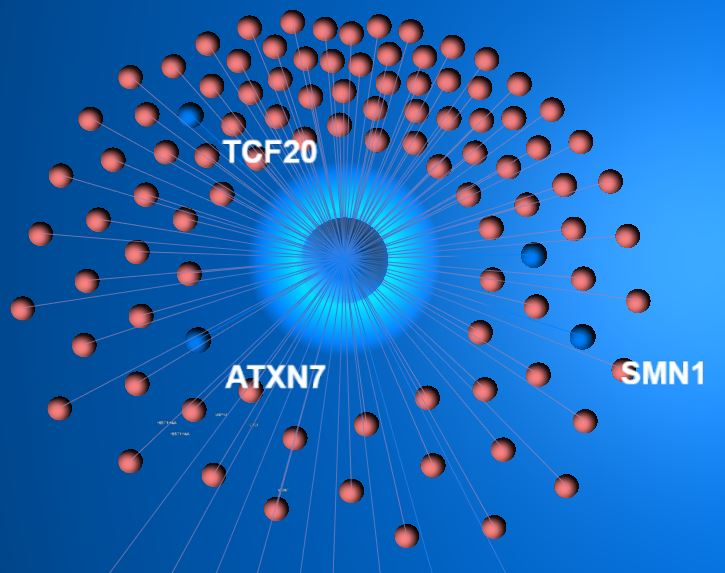
\includegraphics[width=3in]{Hist.JPG}
    }
    \caption{HIST2HAC}
\end{figure}

\section{DISCUSSION AND CONCLUSION}

Searching Uniprot for each protein identified in Fig. 4 and selecting the human variant we were able to identify each of these proteins, their function, and the biological processes in which they are involved. The seed node HIST2H2AC, highlighted in a light blue halo in Fig. 4, was identified as Histone H2A type 2-C which is a component of the nucleosome around which the DNA of chromosomes is wrapped for compaction and to limit accessibility to the machinery of transcription.$^6$ Thus this histone plays an important role in transcription regulation as well as repair, replication and stabilization of chromosomes and the DNA within them.$^6$ The major biological process in which HIST2H2AC is involed is chromatic organization.$^5$. Based on this information we hypothesize that the selected interaction nodes within the HIST2H2AC cluster will play a role in organizing chromatin and the larger nucleus, as well as be involved in activation and execution of transcription.

Human SMN1 was identified as survival motor neuron protein.$^5$ While not as clearly associated as hypothesized, this protein plays a role in catalyzing the assenbly of small nuclear riboproteins (snRNPS), a compoent of the splicosome needed to convert pre-mRNA into the mature, translation ready form.$^6$ It is therefore involved in the transcription process and not contradictory to the hypothesis we formulated. The Uniprot results indicated that a key function of this protein is RNA binding within DNA-template transcription and termination as well as spliceosomal complex assembly processes.$^6$ Interestingly, examining Fig. 4 we see two nodes identified as SMN1, potentially indicating multiple interactions with the histone seed protein.

Human TCF20 was identified as a transcriptional coactivator for the stromelysin gene.$^6$ It therefore strongly supports the hypothesized function of this protein cluster. It was indenitified to have a role in a number of biological functions and processes including DNA-binding and transcription factor activity, RNA binding and regulation of DNA-templated transcroption.$^6$ The third node identified, ATX7, was identified as the human protein ataxin-7 which is a compenent of the STATA transcription coactivator-HAT complex.$^6$ This complex is invovled in histone post-translation modification of histones, thought to be essential to transcription activition and therefore regulation of gene expression. Specifically it plays a role in linking the nuclear cytoskeleton to activated histone complexes and therefore plays an essential role in movement of new transcripts out of the nucleus.$^6$

The results of this analysis show that the identity of a seed node within an cluster can be used as an approximator of associated protein function. It is therefore reasonable to infer the reverse to be true, and placing newly identified protiens in such clusters provide invaluable clues about their identity and function. While our analysis focused on protein-protein interactions, the conclusions should be equally true for the other molecules accepted by OmicsNet. Given this information we can conclude that biological network analysis is an essential tool in mapping the various -omes of the species, aiding scientists in placing novel molecules within the larger web of processes required for biological functioning. Therefore tools such as OmicsNet deserve considerable attention by bioinformatics researchers and dedicating resources to this endeavor will undoubtedly enable discovery and development of products which enhance human and animal well-being.

\addtolength{\textheight}{-12cm}  % This command serves to balance the column lengths
                                  % on the last page of the document manually. It shortens
                                  % the textheight of the last page by a suitable amount.
                                  % This command does not take effect until the next page
                                  % so it should come on the page before the last. Make
                                  % sure that you do not shorten the textheight too much.

%%%%%%%%%%%%%%%%%%%%%%%%%%%%%%%%%%%%%%%%%%%%%%%%%%%%%%%%%%%%%%%%%%%%%%%%%%%%%%%%

\begin{thebibliography}{99}

\bibitem{c1} School of Biological Sciences and Applied Chemistry. (2018). BIF701 Lab 10: Using OmicsNet to Explore Biological Networks. Seneca College: Toronto, ON.

\bibitem{c2} School of Biological Sciences and Applied Chemistry. (2018). Topc 10: Systems Biology. Seneca College: Toronto, ON.

\bibitem{c3} \href{https://dx.doi.org/10.1093%2Fnar%2Fgky510}{Zhou, G., Xia, J. (2018). OmicsNet: a web-based tool for creation and visual analysis of biological networks in 3D space. Nucleic acids research, 46(W1), W514-W522.}

\bibitem{c4} \href{https://dx.doi.org/10.1371%2Fjournal.pcbi.1005771}{Ideker, T., Nussinov, R. (2017). Network approaches and applications in biology. PLoS computational biology, 13(10).}

\bibitem{c5} \href{https://www.omicsnet.ca/faces/docs/FaqView.xhtml}{Xia Lab. (2018). OmicsNet: FAQs [Website]. McGill University: Montreal, QC.}

\bibitem{c6} \href{https://www.uniprot.org/}{National Institute of Health. (N.d.) UniProt [Website]. In \emph{Elixir Core Data Resources}. Germany.}

\end{thebibliography}

\end{document}